\documentclass[11pt]{article} 

% ***********************************************************
% ******************* PHYSICS HEADER ************************
% ***********************************************************
% Version 2
%\usepackage{MnSymbol}
\newtheorem{guess}{Hypothesis}
%\usepackage[b5paper]{geometry}


\usepackage{mathtools}   % loads »amsmath«
\usepackage{empheq}


\usepackage{epsfig}
%\usepackage{mdframed}
\usepackage{tikz}
\usetikzlibrary{scopes}
\usepackage{amsmath}
\usepackage{bm}
\usepackage{amsthm } % Theorem Formatting
\usepackage{amssymb}	% Math symbols such as \mathbb
\usepackage{listings}

\usepackage{graphicx}

%\usepackage{hyperref}
\usepackage{multicol} % Allows for multiple columns

\usepackage{fullpage, float, subfig, verbatim,amsmath, mathrsfs}
\usepackage{fancyhdr}
\usepackage{natbib}
\usepackage{appendix}
\usepackage{alltt}
%%%%
\usepackage{breqn}
\usepackage{fixltx2e}

\sloppy
\definecolor{lightgray}{gray}{0.5}
%%%%
\fancyhf{}
\headsep=20pt

% algorithm
\usepackage{algorithm}
\usepackage{algorithmic}


\usepackage[glenn]{fncychap}
\usepackage{sectsty}
\allsectionsfont{\sffamily\mdseries\upshape} % (See the fntguide.pdf for font help)

%Change the chapte layout
\usepackage{titlesec}
\titlespacing*{\chapter}{0pt}{-50pt}{20pt}
\titleformat{\chapter}[display]{\ttfamily \LARGE\bfseries}{\chaptertitlename\ \thechapter}{20pt}{\Huge}

% Fancy MATLAB-kode:
\usepackage{textcomp}
\definecolor{lbcolor}{rgb}{0.95,0.95,0.95}
\lstset{
%	backgroundcolor=\color{lbcolor},
	tabsize=4,
	rulecolor=,
	language=matlab,
        basicstyle=\scriptsize,
        upquote=true,
        aboveskip={1.5\baselineskip},
        columns=fixed,
        showstringspaces=false,
        extendedchars=true,
        breaklines=true,
        prebreak = \raisebox{0ex}[0ex][0ex]{\ensuremath{\hookleftarrow}},
        frame=single,
        showtabs=true,
        showspaces=false,
        showstringspaces=false,
        identifierstyle=\ttfamily,
        keywordstyle=\color[rgb]{0,0,1},
        commentstyle=\color[rgb]{0.133,0.545,0.133},
        stringstyle=\color[rgb]{0.627,0.126,0.941},
        numbers=left, 
        numberstyle=\tiny, 
        stepnumber=1, 
        numbersep=5pt
}

% equations
\definecolor{myeqcolor}{gray}{0.9}
\newcommand*\mygraybox[1]{%
\colorbox{myeqcolor}{\hspace{1em}#1\hspace{1em}}}

% more equation highlightin
%\usepackage{framed}
\usepackage[framemethod=TikZ]{mdframed}
\usepackage{xcolor}
\surroundwithmdframed[
    hidealllines=true,
    backgroundcolor=black!20,
    skipbelow=\baselineskip,
    skipabove=\baselineskip
]{equation}
\global\mdfdefinestyle{graybox}{%
outerlinewidth=0pt,innerlinewidth=0pt,
outerlinecolor=gray,roundcorner=5pt,
backgroundcolor=gray!27
}

\usepackage{longtable}

%\usepackage[svgnames]{xcolor} % Required to specify font color

\newcommand*{\plogo}{\fbox{$\mathcal{PL}$}} % Generic publisher logo

%----------------------------------------------------------------------------------------
%	TITLE PAGE
%----------------------------------------------------------------------------------------

\newcommand*{\titleAT}{\begingroup % Create the command for including the title page in the document
\newlength{\drop} % Command for generating a specific amount of whitespace
\drop=0.1\textheight % Define the command as 10% of the total text height

\rule{\textwidth}{1pt}\par % Thick horizontal line
\vspace{2pt}\vspace{-\baselineskip} % Whitespace between lines
\rule{\textwidth}{0.4pt}\par % Thin horizontal line

\vspace{\drop} % Whitespace between the top lines and title
\centering % Center all text
%\textcolor{Red}{ % Red font color
{\Huge A TITLE}

\vspace{0.25\drop} % Whitespace between the title and short horizontal line
\rule{0.3\textwidth}{0.4pt}\par % Short horizontal line under the title
\vspace{\drop} % Whitespace between the thin horizontal line and the author name
by \\
\vspace{0.25\drop} % Whitespace between the thin horizontal line and the author name
{\Large \textsc{Simen Andresen}}\par % Author name
\vfill % Whitespace between the author name and publisher text

NTNU
\rule{\textwidth}{0.4pt}\par % Thin horizontal line
\vspace{2pt}\vspace{-\baselineskip} % Whitespace between lines
\rule{\textwidth}{1pt}\par % Thick horizontal line

\endgroup}



\linespread{1.5}




% algorithms
\floatstyle{plain}
\newfloat{myalgo}{tbhp}{mya}

\newenvironment{Algorithm}[2][tbh]%
{\begin{myalgo}[#1]
\centering
\begin{minipage}{#2}
\begin{algorithm}[H]}%
{\end{algorithm}
\end{minipage}
\end{myalgo}}

% then use the following
		%\begin{Algorithm}[t]
		%\caption{Does work, though no nice solution.}
		%\end{Algorithm}

%\newcommand{\textpath}{./texts/}



%%%%%%% TITLE %%%%%%%%%%%%%%%%%%%%%

\title{My title}
\author{Simen Andresen}
\date{\ \\ \ \\ \today}

%%%%%%%%%%% DOCUMENT %%%%%%%%%%%%%
\begin{document}

\captionsetup{width=0.8\textwidth}

% custom commands - variables etc
\newcommand{\bs}{\boldsymbol}
\newcommand{\taub}{\bs \tau}
\newcommand{\vdotbb}{\dot{\bs V}_{0b}^B}
\newcommand{\vdotb}[2]{\dot{\bs V}_{#1}^#2}
\newcommand{\vbb}{\bs V_{0b}^B}
\newcommand{\vb}[2]{\ensuremath{\bs V_{#1}^#2}}
\newcommand{\jg}[2]{\ensuremath{\bs J_{#1}^#2}}
\newcommand{\qdot}{\dot{\bs q}}
\newcommand{\xidotb}{\dot{\bs \xi}}
\newcommand{\xib}{\bs \xi}
\newcommand{\zetab}{\bs \zeta}
\newcommand{\zetadotb}{\dot{\bs \zeta}}
\newcommand{\etab}{\ensuremath{\bs \eta}}
\newcommand{\etadotb}{\ensuremath{\dot{\bs \eta}}}
\newcommand{\adg}[1]{\ensuremath{\bs{Ad}_{g_{#1}}}}
\newcommand{\adgb}{\ensuremath{\bs{Ad}_{g_{0b}}}}
\renewcommand{\frame}[1]{\ensuremath{\mathcal{F}_{#1}}}
\newcommand{\Real}[1]{\ensuremath{\mathbb{R}^{#1}}}
\newcommand{\rb}[1]{\ensuremath{\bs R_{#1}}}
\newcommand{\pb}[1]{\ensuremath{\bs p_{#1}}}
\newcommand{\jb}[2]{\ensuremath{\bs J_{#1}^{#2}}}

\pagestyle{empty}
\titleAT

\
\cleardoublepage



 %%%%%%%%%%%%% BODY %%%%%%%%%%%%%%
\pagestyle{plain}

\pagenumbering{roman} % Roman numerals
\setcounter{page}{1}

\section*{Problem Description}
Ocean space research using underwater robotics is important for mapping, characterization and monitoring of climate and environment, exploration and exploitation of hydrocarbons and other minerals and resources in demanding areas such as deep water and under ice. The main challenge is to increase the level of autonomy and robustness for automatic mapping, monitoring and intervention, high-level planning/re-planning and reconfiguration of single and multiple vehicles subject to the particular mission, environmental condition, available energy, communication constraints, and any failure conditions.

The Centre of Excellence Autonomous Marine Operations and Systems (AMOS) is dedicated to address these control challenges. The center has high expertise and cutting edge experimental facilities to solve the corresponding control problems. This MSc project will be integrated in the AMOS research, with the corresponding access to cutting edge expertise and experimental facilities.

In particular, this MSc project will address the control challenges of underwater robotics. Development of control and optimisation methods for high-level planning/re-planning and reconfiguration of autonomous underwater vehicles with manipulation capabilities operating in various environmental conditions and in confined areas. This involves modelling of the hydrodynamic loads induced on vehicles by the interaction with the sea bottom, risers or other marine units. Varying hydrodynamic models, both in structure and parameters, and their influence on control system design for vehicle and robotic manipulators will be studied. This is necessary due to different tool configurations and modes of operations. For certain repair operations the underwater vehicle may be connected to the subsea template by some umbilical for energy supply and possible tele-robotics functions.
\\
The following subtasks are proposed for this project:
\begin{enumerate}
	\item Perform a literature study on underwater robotics, focusing on AUV/ROVs with manipulator arms attached. To get you started, have a look at Underwater Robots by Antonelli, Springer verlag 2003, and Chapter 10 of Vehicle-manipulator Systems by From, Gravdahl and Pettersen, Springer verlag 2013. Complete the literature study with recent related conference and journal papers on the topic.
	\item Identify/choose a realistic mathematical model of an AUV/ROV-manipulator system. In particular, make sure to include the currents, similarly to Equation (8.147) in Handbook of Marine Craft Hydrodynamics and Motion Control by Fossen, Wiley, 2011. Assume that the current is irrotational and constant.
	\item Develop a force control strategy for the manipulator-AUV/ROV.  Alternative: Develop a control strategy for teleoperation of the manipulator-AUV/ROV system (possibly with a local force control solution). Application: Automated Hot Stab Operation.
	\item Show the effectiveness of the developed control strategy through simulations.
\end{enumerate}

Supervisor: Professor Kristin Y. Pettersen\\
\indent Co-Supervisor: PhD candidate MSc Signe Moe

\clearpage


\section*{Preface}
\noindent This paper constitutes the master project, which is a part of a 5 year study in engineering cybernetics at the Norwegian University of Science and Technology (NTNU). 
It is written during the autumn of 2013, and is a done in collaboration with the Center of Excellence Autonomous Marine Operations and Systems (AMOS) as a part of their research on underwater autonomy. The project is continued as a master-thesis, which will be done during the spring of 2014. 
\bigskip
\bigskip
\bigskip
\bigskip

{
	\centering Trondheim 2013-12-20

}

\bigskip
\bigskip

{
	\centering Simen Andresen

}

\cleardoublepage
\raggedright


\section*{Abstract}
This paper is on the topics of Underwater Vehicle-Manipulator Systems (UVMS). Literature from recent years on this subject is presented and discussed. Further, a model of the kinematics and kinetics of the UVMS is developed based on well known literature, both from the field of robotics and marine dynamics. 

In order to facilitate human interaction with the UVMS, a path correcting control law using force feedback has been proposed in order to deal with compliance of the end effector when interacting with the environment. Also an inverse kinematic control strategy is proposed to deal with the different bandwidth of the vehicle and manipulator and to give less controllable degrees of freedom for human control. Finally, simulations is done with the developed control strategies, yielding a reduction in energy needed to interact with the environment and good path following under ideal conditions.  


\cleardoublepage


\section*{Acknowledgment}
First I would like to thank my supervisor Professor Kristin Y. Pettersen for giving me the opportunity to work on a topic I find so interesting, and for taking the time to have regular discussions on the project. 

\bigskip
\noindent Second I would also like to thank Torstein A. Myhre for help and guidance and help in the field of robotics and computer tools.

\bigskip
\noindent
Finally I would like to thank Nina F. Lillemoen, Hans Erik Froeyen and Marius Vikhammer, who I share my office with, for companionship and discussions on topics relevant to the project.
\bigskip
\bigskip

{ 
	\raggedleft S. A.

}
\cleardoublepage

\section*{Notationand Acronyms}

\subsection*{Acronyms}
%acronyms
    \begin{longtable}{p{6cm}p{10cm}}
		AUV & Autonomous underwater vehicle
		\\
		DH & Denavit-Hartenberg 
		\\
		ROV & Remotely operated vehicle 
		\\
		UVMS & Underwater Vehicle-Manipulator System


    \end{longtable}
\subsection*{Mathematical notation}
%math
%\begin{table}[h!]
    \begin{longtable}{p{6cm}p{10cm}}
			n & Number of links of the manipulator \\
			m & Number of degrees of freedom of the vehicle.  \\
			$\bs J \in \Real{6\times (m+n)}$ & $\bs J$ without superscripts or subscripts is always the jacobian mapping the quasi-velocities $\bs \zeta$ to the body velocity of the end effector\\
			$\bs \omega_{0b} \in \Real 3$ & Rotational velocity of vehicle as observed from body frame.  \\
			$\bs R_{ab} \in \Real{3 \times 3}$ & Rotation matrix representing the rotation of \frame b with respect to \frame a \\
			$\bs J^{\dagger} \in \Real{(m+n) \times 6}$ & Pseudo-inverse of $\bs J$\\
			$\bs V_{0b}^{B} \in \Real 6  $ & Body velocity twist of vehicle\\
			$\bs V_{0b}^{S}\in \Real 6 $ & Spatial velocity twist of vehicle\\
			$\bs V_{0e}^{B}\in \Real 6 $ & Body velocity twist of end effector\\
			$\bs V_{0e}^{S}\in \Real 6 $ & Spatial velocity twist of end effector\\
			$\bs \tau_{c} \in \Real{m+n}$ & Controlled input generalized forces\\
			$\bs \eta = \begin{bmatrix} (\bs \eta_{1})^{T} & (\bs \eta_{2})^{T}\end{bmatrix}^{T} \in \Real 6$  & Position and rotation (euler angles) of the vehicle, relative to an inertial frame \\
			$\bs \eta_{e} \in \Real 6$ & Position and rotation of end effector relative to inertial frame \\ 
			$\bs \xi = \begin{bmatrix} (\bs \eta)^{T} & (\bs q)^{T}\end{bmatrix}^{T} \in \Real {m+n} $ &  Configuration of UVMS \\
			$\bs \zeta = \begin{bmatrix} (\vb{0b}{B})^{T} & (\dot{\bs q})^{T}\end{bmatrix}^{T} \in \Real{m+n}$ & Velocities of the vehicle and manipulator arm. \\
			$\bs J_{a} \in \Real{(m+n) \times (m+n)} $ & Analytical Jacobian. Mapping quasi-velocities to the time derrivative of the general coordinates. \\
			$ \adg{0i}$ & Adjoint map matrix operator. \\
			$\jg{gi}{B} \in \Real{6 \times (m+n)}$ & Geometric Jacobian. Mapping quasi velocities to velocities of frame \frame i\\
			$\jg{ge}{B} \in \Real{6 \times (m+n)}$ & Geometric Jacobian. Mapping quasi velocities to velocities of end effector\\
			$\bs F_{e}^{e} \in \Real 6 $ & Force on end effector from interaction with the environment \\
			$|| \cdot ||$ & The 2 norm operator	 \\
			$|| \cdot ||_{\infty} $ & The infinity norm operator	



			
			

    \end{longtable}
%\end{table}




\clearpage



\cleardoublepage
\tableofcontents
\cleardoublepage

\pagenumbering{arabic} % Roman numerals
\pagestyle{fancy}
\chead{Underwater Robotics}
\rhead{\sectionmark}
\setcounter{page}{1}

\lfoot{\thepage}





\section{Introduction}
\subsection{Background}
In recent years, technological advancement and an increase in interest for underwater recourses has contributed to an increase in manned underwater activity, both for research and for industrial gain. Examples of this is the extraction of oil and gas from reservoirs under the seabed, marine archeology, and underwater mining. In many aspects of underwater activity manned operation is considered difficult, unsafe, inefficient and/or tedious. Therefor, underwater vehicles provides a preferable, and in many cases necessary tool. 

Remotely Operated Vehicles (ROV) have been used for several decades, and consists of an underwater vehicle tethered to a manned control station (e.g. a ship) to provide communication and to close the human-vehicle control loop.  

Autonomous Underwater Vehicles (AUV), on the other hand, should be completely autonomous, and without a tether. An Underwater Vehicle-Manipulator System (UVMS) is a collective term used for both AUV's and ROV's with manipulator capabilities (robot arms). Since both ROV's and AUV's share most of their properties, UVMS will be the generalization which will be used in this paper. 

In order to do complicated tasks, such as intervening  with the environment, ROV's are today the vehicle of choice. For simpler tasks, such as pipeline inspections, it is realistic with fully autonomous vehicles, using well known path following methods and control strategies (see e.g. \cite{fs}).  
Still there is a large gap between ROV's and AUV's when it comes to doing complicated tasks involving e.g. manipulator capabilities. In order to bridge this gap, it is important to look at strategies to keep the human, as much as possible, out of the control loop, and thus providing semi-autonomous control. 

\subsection{Problem Formulation}
An UVMS is a highly dynamic system with complicated kinematics as well as complex kinetics due to high coupling between rigid bodies and hydrodynamics and external influences such as sea current. This paper presents models for the kinematics and kinetics, using a framework from the robotic literature (and also, more recently, from the ship modeling literature).

A hot stab operation is a typical operation for a UVMS where precision is important, and the manipulator interacts with the environment. The hot stab operation, as done today, demands highly skilled operators, and excessively robust tools and structures to withstand the impact between manipulator and environment.  Control methods using measurements of the force on the end effector\footnote{The end effector is the robot gripper or hand, i.e. the last link of the robot manipulator} of the robot is therefor developed. Further, kinematic control methods will be designed, for humans to control only some degrees of freedom (DOFs) of the end effector, yielding higher accuracy.

\subsection{Structure of the paper} 
It is assumed that the reader has some knowledge of robot or ship modeling and control, and is familiar with rigid body dynamics and kinematics. The paper starts with a presentation of recent years' literature on UVMS's in section \ref{sec:literature}. In section \ref{sec:modelling}, the mathematical model is derived and presented.
In section \ref{sec:control} control laws are presented, in section \ref{sec:simulation} the proposed control laws are simulated, and finally in section (sitation needed) a conclusion is made and further work is proposed.

\clearpage
\section{Literature Review}
\label{sec:literature}
In this section, different litterature on the topic of underwater vehicles with manipulators (UVMS) is presented. To focus is mostly on kinematics and force control solutions, but also some general modeling and motion control is presented.  
\\

\subsection{Antonelli G. - Underwater robotics}

\cite{antonelli1} presents mathematical models of the UVMS kinematics and dynamics, as well as motion control strategies for both the vehicle, and the total system, including a manipulator arm. For motion control, several strategies using adaptive control, is presented, where the controller adapts on a minimal set of parameters. Simulations is used to show the effectiveness of both the motion control, as well as for the kinematic control. Mathematical models for well known research UVMS's are used, facilitating the process of compareing control strategies. 
% kinematics

A real-time kinematic control is proposed for the total veichle-manipulator system, exploiting the redundancy in the system. This is generalized for an ROV with the normal 6 DOFs and with a m-link manipulator giving the system a total of $6+m$ DOFs. 
\cite{antonelli1} proposes a Closed-Loop Inverse Kinematic Algorithm for solving the inverse kinematics\footnote{Inverse kinematics will be explained later in this paper. In short it is the process of mapping end effector velocities to vehicle and joint velocities}. The algorithm uses feedback from the resulting position of the end effector to correct for the numerical drift in the method. The inverse velocity kinematics is solved with the following

\begin{align}
\label{eq:antIK}
\bs \zeta_r &=\bs J_{p}^{\dagger}(\bs \eta,\bs q) \left( \dot{\bs x}_{p,d} + \bs K_{e} \bs e_{e} \right) + \left( \bs I_N - \bs J_{p}^\dagger(\bs \eta,\bs q) \bs J_{p}(\bs \eta,\bs q)  \right)\bs J_{s}^\dagger(\bs \eta,\bs q) \left(\dot{\bs x}_{s,d} + \bs K_{s}e_{s} \right)
\end{align}
Where $ \dot{\bs x}_{p,d}$ and  $ \dot{\bs x}_{s,d}$ are the primary and secondary task coordinates, representing the end effector and vehicle velocities respectively. The matrices $\bs J_p$ and $ \bs J_s $ is the mapping from the vehicle and joint positions to the primary and secondary task coordinates. $\bs J^{\dagger}$ is the Moore-Penrose pseudo inverse of $\bs J$. The vectors $\bs K_{e}\bs e_{e}$ and $ \bs K_{s}\bs e_{s}$ are the weighted  position error of the primary and secondary tasks respectively.
The primary task is defined as the planned velocity of the end effector, while the secondary task is the desired motion of some internal element of the kinematics chain, e.g. the vehicle, that does not change the end effector velocity.

\cite{antonelli1} also presents a fuzzy inverse kinematics law, based on the weighted pseudo inverse

\begin{align}
	\bs J_{w}^{\dagger} &= \bs W^{-1} \bs J^{T} \left( \bs J \bs W^{-1}\bs J^{T} \right)^{-1}
	\label{eq:wpseudo}
\end{align}

The weighted pseudo inverse is widely used in robotics, as a robust way of avoiding joint limits by weighting the diagonal elements of $\bs W$ according to how close they are to a limit. In \cite{antonelli1}, the weighing matrix $\bs W$ is used to distribute the motion between the manipulator and the vehicle. This is done in order to avoid unescessary motion of the vehicle, yielding a more energy effective approach, due to the vehicles large inertia, relatice to the manipulator.

% end antonelli

% kim two time scale
\subsection{Kim et al. -  Dynamic Analysis and Two-Time Scale Control for
Underwater Vehicle-Manipulator Systems}

\cite{two_time_scale} proposes a control scheme that takes the different bandwidth of the manipulator and vehichle into account for a generalized UVMS with a $n$-link manipulator. This is favourable since the bandwidth of the vehichle is naturally much lower due to it's larger inertia. The proposed control scheme is an active damping control with two-time scale approach in operational space. The basic consept is to control the vehichle alone using a passive or simply a proportional (P) control, and a two-time scale controller for the manipulator to control the total UVMS. 

The vehichle is represented in a partially linear form, and the vehichle is controlled using
\begin{align}
  \bs \tau_v &= - \bs J_{v}^{-1}(\bs \eta)\bs K_v \bs \eta
  \label{eq:kimProp}
\end{align}
Where $\bs J_v(\bs \eta)$ is defined as $\etadotb=\bs J_v(\etab)\vbb $. By including the controller in the partially linearized dynamics of the UVM system the manipulator control law is proposed as a feedback linearizing controller:
\begin{align}
  \bs \tau_m &=\bs M^* \bs u+ \bs h^*
  \label{eq:kim_feedback_lin}
\end{align}
By including \eqref{eq:kim_feedback_lin} the system yields:

\begin{align}
  \bs M_{11}  \vdotbb + \bs J_v^{-1} \bs K_v \bs \eta &= -\bs M_{12} \bs u
  \label{eq:kim_linearized} \\
  \bs{\ddot q} &=\bs u
  \label{eq_kim_linearized2}
\end{align}
For a definition of the inertia matrices $M_{11}$ and $M_{12}$ the reader are refered to \cite{two_time_scale}. Further the control input $u$ is defined as $\bs u = \bs u_{slow}+\bs u_{fast}$ where the slow part mainly affects the vehichle dynamics, while the fast part mainly affects the manipulator. $\bs u_{fast}$ is then designed as a high gain linear tracking controller yielding a frequency much higher than the bandwidth of the vehichle. The controller scheme is tested on ODIN \footnote{ODIN(Omni-Directional Intelligent Navigator) is a underwater robot developed at the Autonomous Systems Laboratory of the University of Hawaii} with a 3 DOFs manipulator, showing good tracking results.  


\subsection{Fossen et al. - Modeling and Control of Underwater Vehicle-Manipulator Systems }

\cite{foss_schjolberg_modelling} presents a mathematical model of a UVMS system, with an in depth description of most of the hydrodynamic terms. The mathematical model is separates between the manipulator dynamics and the vehicle dynamics by adding the forces of interaction between them.

proposes a control law for the UVM system utilizing feedback linearization. The number of DOFs of the manipulator is not specified, but the refered manipulator jacobian is invertible and it is therefor reasonable to assume a 6 DOFs manipulator. The idea of the controller is to feedback the nonlinear terms acting on the ROV and the manipulator independently, and further use a PID feedback yielding exponential tracking error dynamics in both the manipulator and the vehichle. The proposed controller yields the closed loop control for the vehicle

\begin{align}
	\bs \tau_{r} & = \bs M_{11}(\bs q) \bs a_{v} + \bs M_{c}(\bs q) \ddot{\bs q} + \bs n_{1} \\
	\bs a_{v} &= \ddot{\bs \eta}_{d} - \bs K_{p} \tilde{\bs \eta} - \bs K_{d} \dot{\tilde{\bs \eta}} + \bs n_{1} \left( \bs q, \dot{\bs q},\bs \nu \right)
	\label{eq:fossenfbl}
\end{align}
$\bs n_{1}$ is then the vector containing all the nonlinearities of the vehicle. The control input to the manipulator $\bs \tau_{m}$ is defined in the same way. 



\subsection{Han et al. - 
Redundancy Resolution for Underwater Vehicle-Manipulator Systems
with Minimizing Restoring Moments }

\cite{redundancy_res_restoring_forces} Proposes a redundancy resolution of UVM systems which minimizes the restoring moments. The freedom of motion in the nullspace of the end effector can then be used to position the vehichle in a way that is advantagous to the energy consumption of the UVMS. This is especially favourable when the system is run by battery, and hence minimizing energy consumption is essential.
The proposed inverse kinematic uses the weighted pseudo inverse and projects the vector $z$ into the nullspace of the jacobian $\bs J$ 
\begin{align}
  \xidotb&=\bs J^{W \dagger} \dot{\bs x}_E^0+(\bs I- \bs J^{W \dagger})\bs z
  \label{eq:restoringforces_inverse}  \\
  \bs J^{W \dagger}&= \bs W^{-1} \bs J^T  \left( \bs J \bs W^{-1} \bs J^T \right) ^{-1}
  \label{eq:restoring_J}
\end{align}
Where an arbitrary velocity vector $\bs z\in \mathbb{R}^{6+n}$ is projected in the null space of the end effector Jacobian and $\bs W$ is any positive definite weight matrix, in the same way as proposed in \cite{antonelli1}. 
The vector $z$ is then the gradient projection direction of a cost function $\phi$ which measures the systems performance to minimize the restoring moments of the vehicle. The proposed cost function is

\begin{align}
	\phi &= \frac{1}{2} || \bs r_{g} - \bs r_{b} ||
	\label{eq:minimizingrestoring}
\end{align}
Where the vectors $\bs r_{g}$ and $\bs r_{b}$ are the vectors representing the center of gravity and boyancy, respectively. The paper presents simulation results, yielding good results in saving energy.







\subsection{Yong Cui \& Niljanjan Sarkar - A Unified Force Control Approach to Autonomous}
Underwater Manipulation
\cite{unified_force_control} proposes a unified force control law for an UVM system. The UVM system is generalized for a 6 DOFs underwater vehicle and an 3-link arm. The paper includes a model of the total system, without taking the current effect into account. The controller is based on hybrid force/position and impedance control, and is supposed to keep a stable contact with the environment as well as tracking desired force trajectories without the knowledge of the environment. The paper distinguishes the three phases of operation: 


\begin{itemize}
  \item No contact with environment
  \item Transition phase
  \item Contact with environment
\end{itemize}
Because of the difference of control in the three phases, a fuzzy rule is proposed to identify and switch control between the different phases. The system is modeled in the task space of the end effector motion with pose $\bs X$
\begin{align}
  \tilde{\bs M}\ddot{\bs X}  + \tilde{\bs \zeta} = \bs F - \bs F_e
	\label{eq:unified_model} 
\end{align}
Where $\tilde{\bs \zeta}$ collects the coriolis, hydronanymic and gravitational forces, $\bs F$ and $\bs F_e$ is the controlled force and the force from the environment, respectively. The proposed control $\bs F_c $ is

\begin{align}
  \bs F_c &=\bs F_{IP}W + \bs F_H(1-W )+ \hat{\tilde{\bs \zeta}} + \bs F_e 
  \label{eq:unified_force}
\end{align}
Where $\bs F_{IP}$ is the output of an impedance controller,$\bs F_{H}$ is the output of a hybrid force/position controller, $\hat{\tilde{\bs \zeta}}$ is an estimate of $\tilde{\bs \zeta}$ and $W$ is the weight variable, controlled by the fuzzy logic.

The purpose of the fuzzy law tuning the weight $W$ is to keep a smooth transition between the three states. Especially in the transition phase it is difficult to keep a good model of the UVMS. When the UVMS operates in the no contact phase, it is only controlled with an impedance control which is obtained by $W=1$. The impedance controller is based on the work done in \cite{impedance_stability}, and has the following structure

\begin{align}
  \bs  F_{IP} &= \hat{\tilde{\bs M}}\bs U % \hat{\tilde{\bs \zeta}} + \bs F_e
  \label{eq:impedance_control}
\end{align}
Where the hat operator indicates the estimate of the variables, and $\bs U$ is the commanded acceleration giving the desired impedance:

\begin{align}
  \bs U&=\ddot{\bs X}_d + \bs P^{-1}\left[ \bs B_d(\dot{\bs X}_d-\dot{\bs X}) + \bs K(\bs X_d - \bs X) - \bs F_e\right]
  \label{eq:impedance_control2}
\end{align}
Where $\bs P$, $\bs B_d$ and $\bs K$ gives the desired impedance relationship between the end effector and the environment. Further the hybrid position/force command $\bs F_H$ in \eqref{eq:unified_force} is based on the following

\begin{align}
  \bs F_H&= (\bs I - \bs S)\bs F_p + \bs S \bs F_f
  \label{eq:hybrid1}
\end{align}
Where $\bs S$ is the compliance selection matrix selecting which directions in the task space force control should be applied and which directions position control should be applied. $\bs F_p$ and $\bs F_f$ is the output from PID and PI controllers, controlling the position and force respectively.


The fuzzy rule tunes W according to the state of the system in terms of the ratio of $\frac{\bs F_e}{\bs F_d}$  and $\bs \nu_e$ where $\bs \nu_e$ and $\bs F_d$ is the desired velocity and force at the end effector. 
Numerical simulations are done yielding good results of motion between no contact and contact operations. 





\subsection{Agility for Underwater Floating Manipulation: Task \& Subsystem Priority Based Control Strategy}
The paper from \cite{trident_1} presents interesting results from the control methodology used in the EU-FP7 TRIDENT project. Trident is based on cooperation between an Unmanned Surface Craft(USC), and an AUV with manipulator capabilities, yielding many interesting possibilities especially with respect to navigation. The Trident is aimed to develop a multipurpose Intervention AUV (I-AUV) for used for intervention in unstructured underwater environments (\cite{trident1}).The I-AUV consists of a controlled AUV which constitutes the floating base of a redundant manipulator manipulator.  The main objectives in \cite{trident_1} is to avoid joint limits in the manipulator, to keep the end effector in a dexterous pose visible for the camera, and finally to get the end effector in the position to e.g. grasp an object. This is done by  

\newcommand*{\mybox}[2]{\colorbox{#1!30}{\parbox{.98\linewidth}{#2}}}





\section{Modelling}
\label{sec:modelling}

In this section mathematical models of the UVMS is presented. The kinematics of the UVMS is highly complex due to the mix of quasi-velocities and generalized velocities, and the number of degrees of freedom of the total system. 
The kinetics is also highly complex, due to the high amount of parameters in the hydrodynamics, strong coupling forces between the rigid bodies, varying inertia for different manipulator configuration and the external influences such as sea current. The kinematics can be derived in the framework of Lie groups and Lie algebras. However, a detailed study of this is not included, but can be found in e.g. \cite{bullo1} or \cite{shankar1}. It should be noted that some of the notation is not consistent with the  litterature of underwater vehicles, due to the need to be consistent within the framework of the UVMS when refering to velocities. Instead of refering to the body velocity of the ship as $ \bs \nu$, the notation $ \vb{0b}{B}$ is used in order to comply with the notation used for velocities of the other frames in the UVMS. 



%kinematics
\subsection{Kinematics}
Kinematics describe the dynamics of the system in terms of geometry, without taking into account how the motion is created. To derive the kinematics of an UVMS, one assumes that all the links in the system are perfectly rigid, and the motion of each rigid body is composed of either a translation, a rotation or both. One of the most important properties of a robotic kinematic chain is the velocities, and it is therefor important to have a good definition. For deriving control laws for the system, one is interested in tracking velocities, both for the end effector and the vehicle. Throughout this paper, the velocity of a rigid body  will be described either as \textit{spatial} or \textit{body} velocity twists. The general notation of velocity for a rigid body $i$ is then $\vb{0i}{S}$ or $\vb{0i}{B}$ representing the spatial or body velocity of the \frame i (attached to the rigid body), relative to \frame 0. The linear part of the spatial velocity of a rigid body relative to an inertial frame is the velocity of a point attached to a possible imaginary extension of the body, moving through the inertial frame (\cite{kristin_jant}). The angular velocity part of the spatial velocity, is the angular velocity as seen from the inertial frame. Although somewhat non-intuitive, the spatial representation facilitates the modeling of a multibody kinematic chain (see \cite{featherstone} or \cite{shankar1}) 


\begin{figure}[h!]
  \centering
  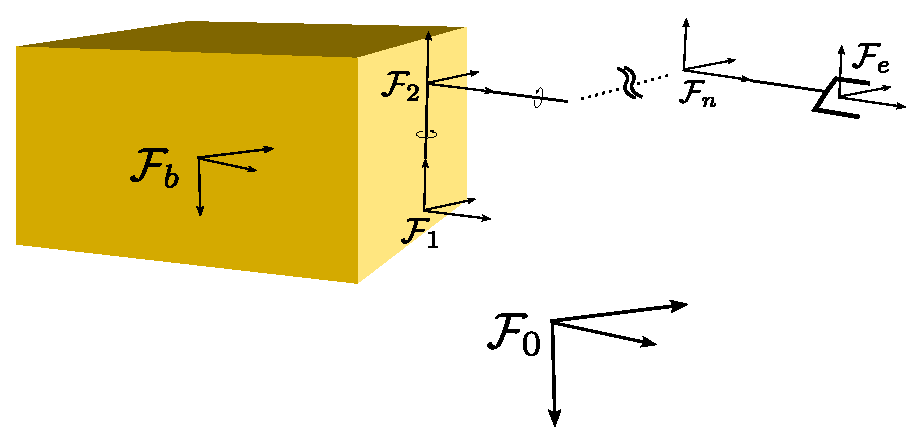
\includegraphics[scale=0.6]{./figures/uvms_kinematics.eps}
  \caption{The assignment of the frames for the UVMS system}
  \label{fig:uvms_kinematics}
\end{figure}
The ROV is regarded as a rigid body with the normal 6 degrees of freedom (DOFs), and the manipulator is a 6-link kinematic chain with only 1 DOF revolute joints. For representing the kinematic structure of the UVM system, a number of frames are assigned as shown in Fig. \ref{fig:uvms_kinematics}. A reference frame $\mathcal{F}_0$ is attached to the earth and is considered inertial. The body frame is located at the ROV's center of mass while the frames of the manipulator is attached according to the Denavit-Hartenburg (DH) convention (\cite{spong2005robot}). 

\begin{figure}[h!]
	\centering
	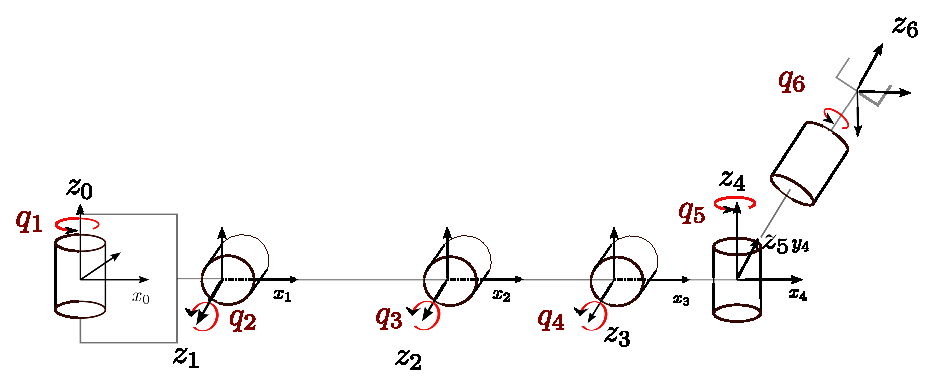
\includegraphics[scale=0.7]{./figures/manipulator_kinematics.eps}
	\caption{The frames are assigned to the kinematic structure of the manipulator according to the DH convention}
	\label{fig:dh-manipulator}
\end{figure}
For representing the orientation of the vehicle euler angles are used, which gives a minimal representation of the attitude at the expense of giving representational singularities, see e.g. \cite{fs}. The position is represented as the coordinates of the origin of $\mathcal{F}_b$ relative to $\mathcal{F}_0$. The configuration of the manipulator are represented using the angles $q$. The total configuration given in generalized coordinates can then be written in vector form.
\begin{align*}
  \xib&:= \left[ \etab^T \bs q^T \right]^T \in \mathbb{R}^{6+n}
  \\
  \etab &= \begin{bmatrix}\etab_1 \\ \etab_2 \end{bmatrix}  = \begin{bmatrix} x_{0b} \\ y_{0b} \\ z_{0b} \\ \phi \\ \theta \\ \psi \end{bmatrix} \in \mathbb{R}^{6}
\end{align*}
One of the challenges to UVM systems is the mix of euclidean and non euclidean transformations representing the configuration of the system. While the transformation of each link is euclidean, the transformation of the vehicle is non-Euclidean \footnote{see e.g. \cite{kristin_jant} for a detailed discussion} , and in general the following is true
\begin{align}
	\bs \omega_{0b} \neq & \etadotb_2
  \label{eq:quasi1}
\end{align}
Thus, the quasi-velocities $ \zetab $ or $\zetab^S$ is used to represent the velocity state of the system
\begin{align}
  \zetab &= \begin{bmatrix} \vbb \\ \qdot \end{bmatrix}
  \label{eq:zeta1}
	\\
	\zetab^S &= \begin{bmatrix} \vb{0b}{S} \\ \qdot \end{bmatrix}
	\label{eq:zetas}
\end{align}
Where $\vbb = \begin{bmatrix} \bs v^{T} & ( \bs \omega_{0b}  )^{T} \end{bmatrix}=  \begin{bmatrix} u & v & w & p & q & r \end{bmatrix}^T \in \mathbb{R}^6 $ is the body velocity twist, and $\zetab^S$ is the corresponding spatial velocities. 

The quasi velocities can be mapped to the time derivative of the generalized coordinates through (\cite{kristin_jant})
\begin{align}
 	\xidotb &=\bs J_a(\etab_2)\zetab 
  \label{eq:quasi_trans}
  \\
  \bs J_a &= \begin{bmatrix} \bs R_{0b}(\eta_2) & 0& 0 \\ 0 & \bs T_{0b}(\eta_2) & 0 \\ 0 & 0 & I \end{bmatrix} \in \mathbb{R}^{(6+n) \times (6+n) }
  \label{eq:jacobian_a}
\end{align}
Where $\bs T_{0b}(\eta_2)$ is written as in \cite{fs}.
\begin{align}
	\dot{\bs \eta}_2 & = \bs T\left( \bs \eta_{2} \right) \bs \omega_{0b}^{b} \\
	\bs T\left( \bs \eta_{2} \right) &= 
		\begin{bmatrix} 1 & s\phi t\theta & c\phi t\theta \\
										0 & c\phi & -s\phi \\
										0 & \frac{s\phi}{c\theta} & \frac{c\phi}{c\theta}
	\end{bmatrix}
	\label{eeq:fossen-transfomrm}
\end{align}
Where $s \; \cdot = sin(\cdot ), \; c \; \cdot = cos(\cdot)$ and $t \; \cdot = tan(\cdot)$. The following is a definition of the total configuration states and velocities


\begin{mdframed}[style=graybox]
\begin{align}
	&\bs \xi \; - \; \text{Generalized coordinates for the UVMS} \nonumber
	\\
	& \zetab \; - \; \text{Quasi velocities for the UVMS in body velocities} \nonumber
	\\
	& \zetab^{S} \; - \; \text{Quasi velocities of the UVMS in spatial velocities} \nonumber
	\\
&	\vb{0e}{B}\; - \; \text{Velocity of the end effector frame \frame e relative to \frame 0 as seen from \frame e} \nonumber
\\
& \vb{0b}{B}\; - \; \text{Velocity of \frame b relative to \frame 0 as seen from the vehicle frame \frame b} \nonumber
\\
&	\vb{0e}{S}\; - \; \text{Velocity of \frame e relative to \frame 0 in spatial coordinates} \nonumber
\\
&	\vb{0b}{S}\; - \; \text{Velocity of \frame b relative to \frame 0 in spatial coordinates} \nonumber
\end{align}

\end{mdframed}
The configuration states are now defined for the total system, together with the mapping between the velocity states and the rate of change of the generalized coordinates through the analytical Jacobian $\bs J_{a}$. Further, it is 
important to define the velocity of frames with respect to an inertial frame, where the velocity of the end effector frame \frame{e} is the most important. This is done through the Geometrical Jacobian $\bs J$, which maps $\zetab \rightarrow \vb{0e}{B}$ or $\zetab^{S} \rightarrow \vb{0e}{S}$  for the body or spatial velocities, respectively. This mapping is derived by using the vehicle velocity twist $\vb{0b}{B}$ (in the case of body velocities) and representing the quasi velocities of the manipulator joints as twists. The process of mapping the link and vehicle velocities to the velocity twist of a frame \frame i is done in several steps. First each relative link velocity $\dot{ q}_{i}$
is represented as a velocity twist by scaling a unit velocity twist by the associated velocity $\dot{q}_{i}$. The unit velocity twist then represent the velocity of a 1 DOF joint represented in the associated link frame. 

Using the notation from \cite{kristin_jant} the body joint twist of a revolute joint is defined as 
\begin{align}
	\bs X_i^i&=\begin{bmatrix} 0&0&0&0&0&1\end{bmatrix}^T
	\label{eq:body_twist}
\end{align}
It should be noted that the twist only has one nonzero component in the angular motion around the z axis due to following the Denavit-Hartenberg (DH) convention. It should also be noted that the body joint twist represents the direction of allowed motion seen from the body of link i, and is therefor always constant.
Next we define the spatial joint twist of a revolute joint as the allowed motion of each link relative to the frame $\mathcal{F}_0$, as written in \cite{kristin_jant}
\begin{align}
	\bs X_i&=\adg{0i}\bs X_i^i
	\label{eq:spatioal_twist}
\end{align}
Where the adjoint transformation of velocity twists between two frames \frame a and \frame b is defined as
\begin{align}
	\adg{ab}  &= \begin{bmatrix} \bs R_{ab} & \widehat{\bs p}_{ab}\bs R_{ab} \\ \bs 0 & \bs R_{ab} \end{bmatrix}
	\label{eq:adjoint}
  \\
	\adg{ab}^{-1} &= \begin{bmatrix} \rb{ab}^T & - \rb{ab}^T \widehat{\bs p}_{ab} \\ 0 & \rb{ab}^T \end{bmatrix}
	\label{eq:adjoint2}
\end{align}
Where \rb{ab} is the rotation matrix from \frame{a} to \frame{b}, and \pb{ab} is the vector representing the linear displacement of the origin of \frame b wrt. to \frame a. It should be noted that \adg{ab} can be seen as a transformation from body velocity \vb{ab}{B} to spatial velocity \vb{ab}{S}.
The hat operator $\widehat{(\cdot)}$ maps a vector to it's skew symmetric matrix representation, and when operating on a vector $\bs \omega \in \mathcal{R}^3$ is defined as
 \begin{align}
   \widehat{\bs \omega}&= \begin{bmatrix} 0 & -\omega_3 & \omega_2 \\ \omega_3 & 0 & -\omega_1 \\ -\omega_2 & \omega_1 & 0 \end{bmatrix} 
   \label{eq:skewsym}
 \end{align}
Using  \eqref{eq:adjoint} and \eqref{eq:body_twist} we get

\begin{align}
	\bs X_i&=\begin{bmatrix}\rb{0i} & \widehat{\bs p}_{0i} \rb{0i} \\ \bs 0 & \rb{0i}^T \end{bmatrix}\bs X_i^i
	\label{eq:adjoint_calc}
	\\
	&= \left[\begin{smallmatrix}{}r_{11} & r_{12} & r_{13} & p_{2} r_{31} - p_{3} r_{21} & p_{2} r_{32} - p_{3} r_{22} & p_{2} r_{33} - p_{3} r_{23}\\r_{21} & r_{22} & r_{23} & - p_{1} r_{31} + p_{3} r_{11} & - p_{1} r_{32} + p_{3} r_{12} & - p_{1} r_{33} + p_{3} r_{13}\\r_{31} & r_{32} & r_{33} & p_{1} r_{21} + p_{2} r_{11} & p_{1} r_{22} + p_{2} r_{12} & p_{1} r_{23} + p_{2} r_{13}\\0 & 0 & 0 & r_{11} & r_{12} & r_{13}\\0 & 0 & 0 & r_{21} & r_{22} & r_{23}\\0 & 0 & 0 & r_{31} & r_{32} & r_{33}\end{smallmatrix}\right]
	\left[  \begin{smallmatrix}0\\0\\0\\0\\0\\1 \end{smallmatrix}  \right]
	\\
	&=\left[\begin{smallmatrix}{}p_{2} r_{33} - p_{3} r_{23}\\- p_{1} r_{33} + p_{3} r_{13}\\p_{1} r_{23} + p_{2} r_{13}\\r_{13}\\r_{23}\\r_{33}\end{smallmatrix}\right]
\end{align}
Next we want to find a map from the generalized and quasi velocities to the velocities of each frame $\mathcal{F}_i$ with respect to the inertial frame \frame 0 in spatial coordinates. We also note the mapping between spatial and body velocities
\begin{align}
	\bs V_{0i}^S &=  \adg{0i} \bs V_{0i}^B  
  \label{eq:adg0b1}
 \end{align}
Following the notation in \cite{kristin_jant} we write the mapping from the velocities $\zetab$ to the velocities of frame $\mathcal{F}_i$ in both spatial and body coordinates
\begin{align}
	\vb{0i}{S}&= \jb{gi}{S}(\xib)\zetab^S
  \label{eq:spatial_jacobi}
  \\
	\jb{gi}{S}(\xib) &= \begin{bmatrix} \adg{0b} & \adg{0b} \bs J_i\end{bmatrix}
  \label{eq:spatial_jacobi2}
	\\
	\vb{0i}{B}&= \jb{gi}{B}(\xib)\zetab
  \label{eq:body_jacobi}
  \\
	\jb{gi}{B}(\xib) &= \begin{bmatrix} \adg{bi}^{-1} & \adg{bi}^{-1} \bs J_i\end{bmatrix}
  \label{eq:body_jacobi2}
\end{align}
Where $\bs J_i$ is the spatial geometric Jacobian of link i as written in \cite{kristin_jant} mapping the joint velocities to the spatial twist of link $i$
\begin{align}
  \bs V_{bi}^S &=\bs J_i(q)\dot q
  \label{eq:mappint1}
	\\
	\bs J_i&=\begin{bmatrix}  \bs X_1 & \bs X_2 & \cdots & \bs X_i & \bs 0_{6 \times (n-i)}    \end{bmatrix}
	\label{eq:Ji}
\end{align}
From \eqref{eq:spatial_jacobi} and \eqref{eq:body_jacobi} we get that the end effector velocity can be described using the following
\begin{align}
	\vb{0e}{S} &= \jb{ge}{S}\zetab^S
	\label{eq:ee_velo}
	\\
	&=\begin{bmatrix} \adg{0b} & \adg{0b}\jb{n}{}\end{bmatrix}\zetab^S
	\\
	\vb{0e}{B} &= \jb{ge}{B}\zetab
	\label{eq:ee_velo_body}
	\\
	&= \begin{bmatrix} \adg{bi}^{-1} & \adg{bi}^{-1} \bs J_n\end{bmatrix}\zetab
\end{align}
Where \jb{n}{} is defined in \eqref{eq:Ji} with $i=n$. We can now summarize the velocity kinematics


\begin{mdframed}[style=graybox]
	\begin{align}
	\zetab^S&=\begin{bmatrix} (\vb{0b}{S})^T & (\qdot)^T \end{bmatrix}^T \\
	\zetab^B&=\begin{bmatrix} (\vb{0b}{B})^T & (\qdot)^T \end{bmatrix}^T \\
	\vb{0i}{S}&=\adg{0i}\vb{0i}{B}\\
	\vb{0e}{S}&=\jb{ge}{S}\zeta^S \\
	\vb{0e}{B}&=\jb{ge}{B}\zeta^B \\
	\jb{ge}{S}&=	\begin{bmatrix} \adg{0b} & \adg{0b}\jb{n}{}\end{bmatrix} \\
	\vb{0e}{B}&= \begin{bmatrix} \adg{bi}^{-1} & \adg{bi}^{-1} \bs J_n\end{bmatrix}
\end{align}
\end{mdframed}
%dynamics

\subsection{Kinetics}
The kinetics of the UVMS describes the relationship between the forces and the corresponding motion of the system. The mathematical models describing the motion can be described through Newtons law of motion $F=ma$. As customary in modelling of ship dynamics and robotics, the equations of motion is derived from the knowledge of the total energy of the system using the Lagrangian $L$
\begin{align}
	L=T-V
	\label{eq:lagrange}
\end{align}
Where $T$ and $V$ is the kinetic and potential energy, respectively. Due to the high number of states of the system, the equations of motion are presented in a matrix form, adopted from the robotics litterature, which also has been customary in modern litterature on marine craft modeling and control. First, the equation of motion of the sole vehicle is presented, before the total system, including the manipulator is described.

\subsubsection{Vehicle Dynamics}

A model of a marine craft is proposed in \cite{fs} 

% fossens equations
\begin{align}
\bs M_{RB}\dot{\bs V}_{0b}^B + \bs C_{RB}(\bs V_{0b}^B)\bs V_{0b}^B + \bs g(\bs \eta) + \bs g_0 + \bs M_A \dot{\bs V}_{r}^B  + \bs C_A(\bs V_{r}^B) \bs V_{r}^B + \bs D(\bs V_{r}^B)\bs V_{r}^B = \bs \tau + \bs \tau_{wind} + \bs \tau_{wave} 
\label{eq:fossen1}
\end{align}
Where $ \bs V_{r}^B = \bs V_{0b}^B - \bs V_c^{B}$ is the velocity of the vehichle relative to the water surrounding it, and $ \bs V_{c}^{B}$ is the irrotational current as observed from $\mathcal F_b$. Using the equation in \cite{fs} with a slight change of notation, the equation of the current yields

\begin{align}
	\bs V_c^{B}&=\begin{bmatrix} u_c & v_c & w_c & 0 & 0 & 0\end{bmatrix}^T 
  \label{eq:current}
  \\
  &= \begin{bmatrix} \bs v_c^b & 0 & 0 & 0 \end{bmatrix}^T
  \\
  \bs v_c^0 &= \bs R_{0b}\bs v_c^b 
	\label{eq:current-rotation}
  \\
  \dot{\bs v}_c^i&=0
\end{align}
Where $v_{c}^{0}$ is the constant linear current as observed in the inertial frame \frame 0. It should be noted that since the rotation matrix in \eqref{eq:current-rotation} in general is time varying, the current velocity as observed in the body frame is also time varying. 

Using the properties of an irrational constant current \cite{fs} 
\begin{align}
  \bs C_{RB}(\bs V_{r}^B) &= \bs C_{RB}(\bs V_{0b}^B) 
  \label{eq:irrational}\\
\end{align}
The equation of motion can be written as 
\begin{align}
  \bs M \dot{\bs V}_r + \bs C(\bs V_{r}^B)\bs V_r + \bs D(\bs V_{r}^B)\bs V_{r}^B +  \bs g(\bs \eta) + \bs g_0  &= \bs \tau + \bs \tau_{wind} + \bs \tau_{wave} 
  \label{eq:fossen2}\\
  \bs M &= \bs M_{RB} + \bs M_A
  \label{eq:massCol} \\
  \bs C(\bs V_r^B) &= \bs C_{RB}(\bs V_r^B)+ \bs C_A(\bs V_r^B)
\end{align}


% full UVMS dynamics
\subsubsection{Vehicle Manipulator Dynamics}
The dynamics for the veichle can be included in the total dynamics of the UVMS. As the operation of the UVMS is modelled as being totally submerged, the wind will be removed from \eqref{eq:fossen2}, and the force from waves will be neglected, which is reasonable since the operation will mostly take place in sufficiently deep waters.

Each link of the manipulator can be modelled as a rigid body according to \eqref{eq:fossen2} but looking at the coupled dynamics of the rigid bodies the inertia matrix $\bs M$ is no longer constant but varies with the configuration $\bs q$. The generalized coordinates and generalised and quasi velocities can be written in two separate variables

\begin{align}
  \xib  & := \left[ \bs \eta^T \bs q^T \right]^T
  \label{eq:xi} \\
  \zetab & := \left[ (\vbb)^T \qdot^T \right]^T
  \label{eq:zeta}
\end{align}
and the dynamics of the total system is written in \cite{antonelli1} as

\begin{align}
  \bs M(q)\zetadotb + \bs C(q,\zetab) \bs \zeta +\bs D(q,\zetab) + \bs N(\xib)=\taub
  \label{eq:antonelliDynamics}
\end{align}
where $\bs N(\xib)$ is the gravitational and boyancy forces acting on the vehicle and manipulator. In \eqref{eq:antonelliDynamics} the current is not included in the dynamics, and the author proposes a model in the same form as \eqref{eq:fossen1} with separated rigid body and hydrodynamic terms:

\begin{align}
  \bs M_{RB}\zetadotb+ \bs C_{RB}(\zetab)\zetab + \bs g(\bs \eta) + \bs g_0 + \bs M_A \zetadotb_r  + \bs C_A(\zetab_r) \zetab_r + \bs D(\zetab_r) \zetab_r = \bs \tau 
  \label{eq:withinteraction}
\end{align}
Where $\zetab_r = \begin{bmatrix} (\bs V_r^B)^T & \qdot^T  \end{bmatrix}^T$ is velocity of the system relative to the current. Note that it is sufficient that the vector $\zetab_r$ includes only the relative motion of the vehicle, since the kinematic chain of the manipulator moves relative to the vehichle. Since the current is irrotational and constant the contribution of the linear velocity of the vehicle adds the hydrodynamic terms caused by the current. 

Since the UVMS uses the end effetor to interact with the environment, it is important to include the generalized forces due to contact between the end effector and the environment. Using \cite{spong2005robot} we get the contribution from the interaction forces projected on the generalized forces using the geometric Jacobian $\bs J_{ge}^B$ through the relationship

\begin{align}
  \bs \tau&= (\bs J_{ge}^B)^T \bs F 
  \label{eq:jacobian_force}
\end{align}
Where $\bs F= [f_x, f_y, f_z, n_x, n_y,n_z]^T  $ is the vector of forces and moments from the environment to the end effector. We can then include the interaction forces to the total dynamics
{\small
\begin{mdframed}[style=graybox]
\begin{align}
  \bs M_{RB}\zetadotb+ \bs C_{RB}(\zetab)\zetab + \bs g(\bs \eta) + \bs g_0 + \bs M_A \zetadotb_r  + \bs C_A(\zetab_r) \zetab_r + \bs D(\zetab_r) \zetab_r =\bs \tau+ (\bs J_{ge}^B)^T \bs F 
\label{eq:dyn_with_current}
\end{align}
\end{mdframed}
}




























\section{Control}

\subsection{intro}
Today, this kind of operation is done by maneuvring the vehicle to a position where the manipulator is within reach of the hot stab. Once the desired vehicle position is reached, the vehicle is kept stationary by using dynamical positioning, and another operator operates the manipulator arm to do insert the hot stab. The manipulator is normally controlled through a master-slave configuration,\footnote{A master-slave configuration is a control method where an operator moves a replica of the real manipulator. The obtained angles of the replica is then used by the motion control of the manipulator to obtain the same pose as the replica.} 
or through controling the rates of the joints directly. Both these methods suffer from the following drawbacks:

\begin{itemize}
	\item The operator is dependant on high video feedback with very low latency in order to make the correct adjustments of the manipulator.  
	\item Two operators are normally required, one for the vehicle and one for the manipulator arm.
	\item One has to switch between maneuvring the vehicle and the manipulator, even for tasks that are fairly close to eachother, potentially using more energy then required by the task itself. 
	\item Interaction with the environment is difficult due to latency in force feedback from the manipulator, and difficulty in estimating the forces caused by the interaction.
\end{itemize}
One of the objectives of the control strategy is to keep the human operator out of the control loop as much as possible. This makes the system less dependant on high speed telemetry which is important when operating nontethered vehicles, making it possible to control them from a great distance. 
The proposed control structure is based on controlling the motion of the end effector seen from the end effector frame \frame{ee}. Kinematically this will be done by an inverse kinematic strategy mapping the end effector velocities 
to joint, and vehicle velocities, which will be discussed later. This gives the operator the opportunity to ``fly'' the end effector, without dealing with the rest of the manipulator or the vehicle, as this is being managed locally by the control system. 
Lets now identify the main states of operation of the UVMS, which is useful when designing the control system. 

\begin{itemize}
	\item Transport. This state represent the relatively long distance transport of the UVMS to and from a location where it operates, or when doing inspections of e.g. pipelines. This state requires relatively low accuracy in guidance and is typically done by maneuvering the vehicle only. This can be employed by a classical path following guidance scheme. (See e.g. \cite{fs})  
	\item Repositioning between operation points. In this state, the operator or a path following guidance system will ``fly'' the end effector from one operation point to another, covering relatively short distances. In this state the end effector is controlled and adjusted by an operator controlling the velocities of the end effector.
	\item End effector interaction. The manipulator is used to interact with the environment, for example in a hot stab operation. In this state, high accuracy is required, and should be automatically regulated locally, giving the operator control over the directions of no contact.
\end{itemize}
Before continuing with the force control, a discussion of path following and accuracy is needed. In the two first states the vehicle or the end effector is following a path given by an operator, a path following guidance scheme, or both. The accuracy of the position relative to the desired path is then controlled by the operator through video feedback, or through a guidance system (such as the LOS Guidance Law. See e.g. \cite{fs}). In both cases the guidance is done at a relatively low bandwith, making the path following prone to disturbances, and hence causing the actual path to deviate from the desired path. It is assumed that the reference given to the low level motion control is given as the generalized and quasi velocities of the joints and vehicle. When interacting with the environment the position of the end effector needs to be position controlled at a relatively high bandwidth. This is important in order to be robust to disturbances, and avoid undesired forces on the end effector. To maintain a high bandwidth on the position control, it is recommended that this is done locally, keeping the human out of the position control loop.

A generalized control strategy for the two last states above will now  be proposed, and will later be specified for a hot stab operation. The overall control structure is illustrated in Fig. \ref{fig:control_structure}. Lets now define the desired path given by the operator as $\bs V_{ee,0}$ and $\bs \eta_{ee,0}$. In the second state of operation, only the desired velocity $\bs V_{ee,0}$ is used to specify the desired trajectory. The high bandwidth motion of the end effector is given as $\bs V_{ee,c}$. In the second state we use that 
$$\bs V_{ee,0} = \bs V_{ee,c} $$ 
In the case of the second state of operation the desired velocities of the end effector is mapped, through the inverse kinematics, to reference velocities $\bs \zeta_{c}$ used in the low level motion control.
\begin{figure}[h!]
	\centering
	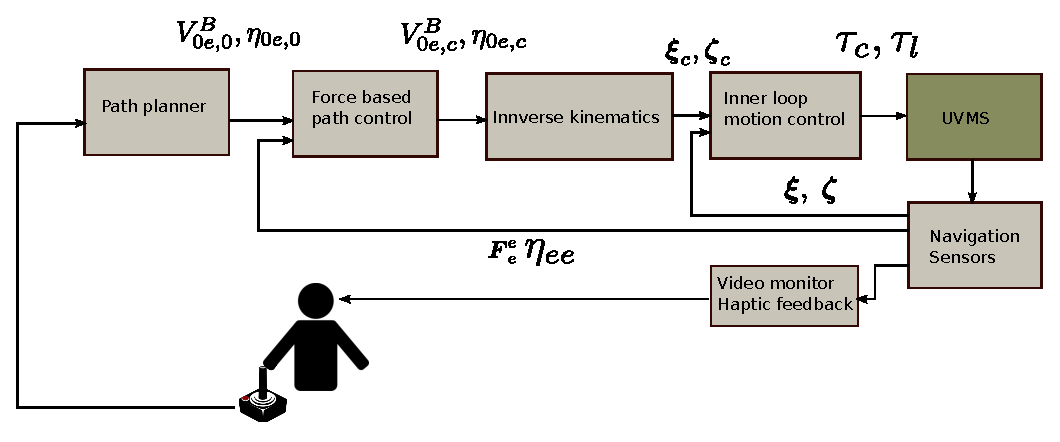
\includegraphics[scale=0.9]{./figures/control_structure.eps}
	\caption{Control structure}
	\label{fig:control_structure}
\end{figure}
In the third state of operation accurate position control is essential, and another approach is therefor proposed specifically for a hot stab operation in the test case below. 

\subsection{Motion Control}
The inner loop of the motion control is outside the scope of this text. For modelling and simulation purposes however, a control strategy based on feedback linearization is proposed, and implemented in SIMULINK in order to 
simulate the force control and the inverse kinematics. To simplify the implementation and analysis we use the model of the UVMS from \eqref{eq:dyn_with_current} split the input $\bs \tau$ into a cancelling term $\bs \tau_c$ and a 
linear control term $\bs \tau_l$ and use $\bs \tau_c$ to cancel out all the nonlinearities and terms including the current, similar to the control law proposed in \cite{foss_schjolberg_modelling}. The nonlinear canceling term yields

\begin{align}
\bs	\tau_{c} &=
  \bs C_{RB}(\zetab)\zetab + \bs g(\bs \eta) + \bs g_0 + \bs M_A \zetadotb_r  + \bs C_A(\zetab_r) \zetab_r + \bs D(\zetab_r) \zetab_r 
	\label{eq:nonlinear-cancelling}
\end{align}
While the linear control term is simply given as

\begin{align}
	\bs \tau_{l} & =\bs M(\bs q) \left(\bs K_{p} \tilde{\bs \zeta} + \dot{\bs \zeta}_{c} \right) \\
	\label{eq:linfeedback-lin}
	\tilde{\bs \zeta} &=\left(\bs \zeta_{c} - \bs{ \hat \zeta } \right)
\end{align}
Where $\bs{ \hat \zeta } $ is the measured or estimation of $\bs \zeta$, and $\bs K_{p}$ is a positive definite matrix. The resulting closed loop dynamics of the UVMS and low level control then yields
\begin{align}
	\bs M(\bs q)_{RB}\zetadotb =\bs M(\bs q) \left(\bs K_{p} \tilde{\bs \zeta} + \dot{\bs \zeta}_{c} \right) + (\bs J_{ge}^B)^T \bs F_{ee}
	\label{eq:linearized_feedback}
\end{align}
As long as there is no contact, the system is stable. This can be proved by looking at the error dynamics of the closed loop system \eqref{eq:linearized_feedback} for $\bs F_{ee}=0$.
\begin{align}
	\dot{\tilde{\bs \zeta}} & =- \bs K_{p} \tilde{\bs \zeta} 
	\label{eq:errordynamics}
\end{align}
Yielding asymtotic stability of the error.
It should be noted that the controller is only proposed for simulation purposes, in order to capture some of the dynamics of the system. Obtaining exact estimates of the nonlinear terms in \eqref{eq:nonlinear-cancelling} is, however, very difficult in real life, and it is thus difficult to guarantee stability.











\subsection{Kinematic Control}
An UVM system is kinematically redundant, meaning that it's configuration space is larger then the task space of the end effector. This is due to the 6 degrees of rotational and translational degrees of freedom of the underwater vehicle in addition to the degrees of freedom given by the number of manipulator joints. Because of this, each configuration of the end effector task space can be obtained by an infinite of configurations in the configuration space of the manipulator. 
As has been customary in robotics litterature, the mapping from the configuration space to the task space of the end effector\footnote{The task space is used to describe the configuration of the end effector relative to an inertial frame.} is done through the Jacobian, mapping the quasi-velocities of the system to the velocities of the end effector as described in \eqref{eq:body_jacobi}. The velocities can then be transformed to the time derivative of the general 
velocities, according to the analytical jacobian \eqref{eq:jacobian_a}, and then integrated to obtain the configuration $\bs \xi(t)$.

\begin{figure}[h!]
	\centering
	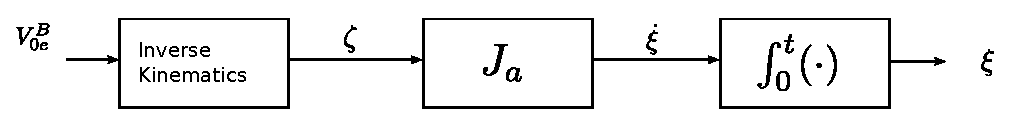
\includegraphics[scale=0.7]{./figures/inverse-kinematics1.eps}
	\caption{Transformation from end effector velocities to generalized coordinates of the UVMS}
	\label{fig:inverse1}
\end{figure}
The inverse kinematics is, in this context, described as the process of obtaining feasible quasi-velocities $\zeta$ from the desired end effector velocities. Due to the redundancy of the system, the set of feasible velocities $\zeta$ is not unique. In robotics litterature the Gradient Projection Method (GPM) is widely used in order to solve inverse kinematics. This method was first proposed in \cite{Liegeois1977}, and has later been developed and adapted my others.
Using the notation in this text, GPM by the following equation (\cite{Liegeois1977})

\begin{align}
	\bs	\zeta	&= \bs J^{+}\vb{0e}{B} + \left( \bs I -\bs J^{+} \bs J \right)k \nabla H
	\label{eq:gpm1}
\end{align}
Where the matrix $\bs J$ is the body geometric jacobian, as described in \eqref{eq:ee_velo_body}, and $\bs J^+ \in \Real{12\times 6}$ is the Moore-Penrose pseudo inverse of $\bs J$. $\left( \bs I - \bs J^{+}\bs J\right)$ projects the velocity matrix $k \nabla H$ into the null space of the jacobian. The vector $k \nabla H$ then describes the inner motion of the system, e.g. the motion that does not change the pose of the end effector (\cite{Liegeois1977} ).
Further, the vector $\nabla H$ is the gradient of a scalar cost function $H$ which is a measure of some performance criterion. For robot manipulator control, $H$ is typically used to avoid joint limits. The null projection of $\nabla H$
can be regarded as an inexact local solution to an optimization problem, where H is a convex function with $\bs \xi$ as the descicion variables. By choosing the gradient direction $\nabla H$ in the configuration space $\bs \xi$, as the null projected velocities gives an effective way of computing velocities to obtain the desired inner motion. The problem with GPM is that not all step lengths in the gradient direcion $\nabla H$ gives a feasible solutions (e.g. keeping the joint commands within the allowed joint limits). Therefore, the parameter k needs to be tuned to give a feasible solution. An efficient and robust method for scaling k is given in \cite{5723588} yielding

\begin{align}
	k&= - \frac{V_{m} - || \bs J^{+}\vb{0e}{B}|| }{||(\bs I - \bs J^{+}\bs J|| ||\left(\bs I - \bs J^{+}\bs J \right) \nabla H||} 
	\label{eq:k-scaling}
\end{align}
Where $V_{m}=||\bs \zeta_{max}||_{\infty}$, i.e. the absolute value of the largest allowed joint velocity of any joint. 




\subsection{Force Control}

Although no control method based on explicit force or impedance control is designed, it is useful to look at the forces of interaction between the end effector and the environment.
The forces on the end effector and the environment is analyzed in the task space, as observed by the end effector. Let the following define the forces in the end effector frame 
\begin{align}
	\bs F_{e}^e&=\begin{bmatrix} f_x & f_y & f_z & m_x & m_y & m_z \end{bmatrix}
	\label{eq:force_force}
\end{align}
$\bs F_{e}^e$ is therefor the same as $\bs F$ defined in \eqref{eq:jacobian_force} and can thus be mapped into the general forces $\taub$ by the transpose jacobian
\begin{align}
	\taub&=(\jb{ge}{B})^T\bs F_{e}^e
	\label{eq:jacobian-force2}
\end{align}

In robot manipulator control, it is customary to control the force between the end effector and the environment, either through direct force control or through controlling the apparent impedance between the end effector and the environment. This is typically done through hybrid impedance/force control, where the end effector is supposed to track a position or a force trajectory each in a subspace of the configuration space of a task frame \frame t. 
A typical application of this is a manipulator washing a car window, where the end effector is position controlled in the plane tangent to the window, while being impedance controled in the direction normal to the window. 
This kind of control scheme requires a priori knowledge of the geometry and environment impedance, and is thus challenging for a UVMS working in a generally unstructured environment. 
A control strategy which does not rely of this a priori knowledge is therefor proposed later in the paper.



























\subsection{Test Case: Semi Autonomous Hot Stab Operation}
A hot stab is a typical operation done by ROV's on subsea installations, which gives the opportunity to connect and disconnect different hydraulic components. 
The hot stab operation is in many ways analogous to the ``peg-in-hole'' problem which is widely studied in robotics litterature. The terms peg and hole will from now on refer to the hot stab tool, and the hole it is inserted into. 
Today, hot-stab is typically done by an operator controlling all of the degrees of freedom of the end effector, or directly in the joint space of the manipulator. This leads to difficulty in putting the peg in the hole, ecpecially 
with large delays in the human-UVMS-loop. 
The proposed strategy in this section is to lock most of the degrees of freedom to position set-points, and let the operator control a minimal set of DOFs. A fuzzy rule will handle the position set-points when the end effector is in 
contact with the environment. The concept is illustrated in Fig. \ref{fig:hot_stab2}.


\begin{figure}[h!]
	\centering
	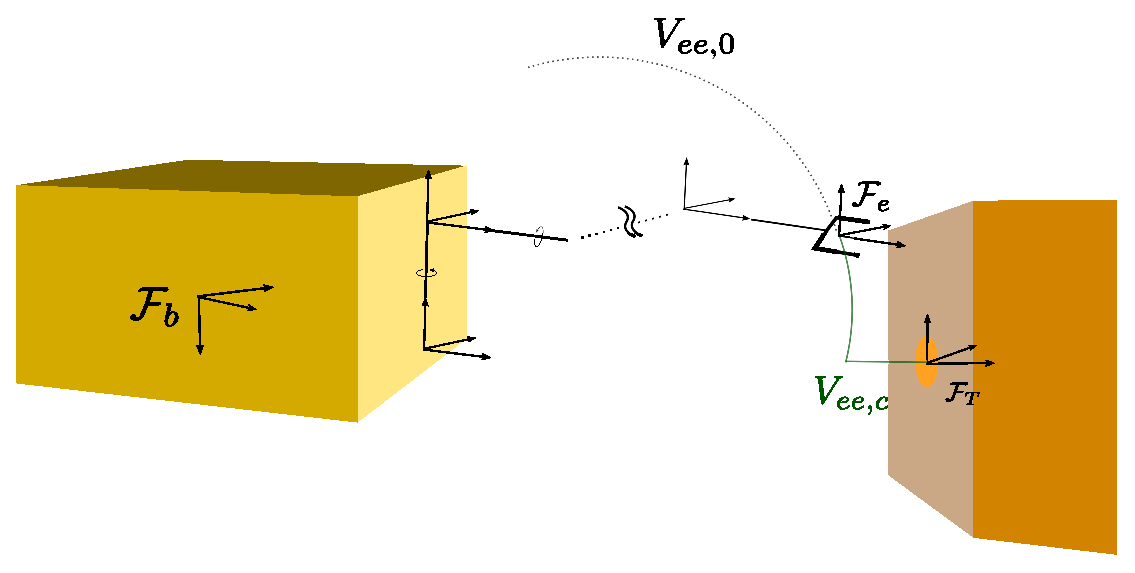
\includegraphics[scale=0.7]{./figures/uvms_hot_stab2.eps}
	\caption{Illustration of the UVMS in the transition between an operator ``flying'' the end effector according to $\bs V_{ee,0}$, and being position controlled in the $z,y,\theta $ and $ \psi$ direction in order to align with the task frame \frame t}
	\label{fig:hot_stab2}
\end{figure}
Further the sets $C$ and $NC$ are defined as

\begin{align*}
	C&=\{y_{ee},z_{ee},\theta_{ee},\psi_{ee}\} - \text{Compliant pose variables}
	\\
	NC&=\{x_{ee},\phi_{ee}\} \; \; \; - \; \text{ Non-Compliant pose variables}
\end{align*}
Where the pose variables above refer to the pose of \frame{ee} relative to the inertial frame. Further, the set-points $\bs \eta_{ee,0}$, given by the operator are good approximations to the pose of \frame{t} given in the inertial frame. Without loss of generality \frame{t} will be used as the inertial frame, and therefor the set-points are given as  
\begin{align}
C \subseteq	\bs \eta_{ee,0}=0
	\label{eq:subset}
\end{align}
A simple outer loop control law is proposed in order to assign a proper commanded velocity variables to the inverse kinematic control, and further, to the low level motion control

\begin{align}
	\bs V_{ee,c} &= \bs K_{1}\bs V_{ee,0} + \alpha \left( \bs F_{ee} \right) \bs K_{2} \tilde{\bs \eta}_{ee} 
	\label{eq:control_law1}
	\\
	\alpha &\in \left[ 0,1\right]
	\\
	\bs K_{1},\bs K_{2}&\in \Real{6 \times 6} \\
	\tilde{\bs \eta}_{ee,0}&= \bs \eta_{ee,0} - \widehat{\bs \eta}_{ee}
\end{align}
Where $\widehat{\bs \eta}_{ee}$ is the estimated or measured pose of the end effector. The matrices $\bs K_{1}$ and $ \bs K_{2}$ are positive semi-definite selection matrices, which selects the variables corresponding to $C$ and $NC$. $\bs K_{2}$ also weighs the contribution of the pose error.  

\begin{align}
	\bs K_{1} =\left[\begin{matrix}{}1 & 0 & 0 & 0 & 0 & 0\\0 & 0 & 0 & 0 & 0 & 0\\0 & 0 & 0 & 0 & 0 & 0\\0 & 0 & 0 & 1 & 0 & 0\\0 & 0 & 0 & 0 & 0 & 0\\0 & 0 & 0 & 0 & 0 & 0\end{matrix}\right]
	\label{eq:k1k2} \; , \; 
\bs K_{1} &=
\left[\begin{matrix}{}0 & 0 & 0 & 0 & 0 & 0\\0 & k_{22} & 0 & 0 & 0 & 0\\0 & 0 & k_{23} & 0 & 0 & 0\\0 & 0 & 0 & 0 & 0 & 0\\0 & 0 & 0 & 0 & k_{25} & 0\\0 & 0 & 0 & 0 & 0 & k_{26}\end{matrix}\right]
\end{align}
The scalar function $\alpha$ are weighting the last term in \eqref{eq:control_law1} based on a fuzzy rule described later. Taking $\alpha = 1$, the control law in \eqref{eq:control_law1} acts as a PI controller on the end effector velocity $\bs V_{ee}$. Where the pose is regarded as the integral of the velocity. Although this is not true in general, since the angular velocities $p_{ee}, q_{ee}$ and $r_{ee}$ in  $\bs V_{ee}$ are quasi-velocities, it can be shown that it is a good approximation close to the end effector pose $\phi_{ee} = \theta_{ee}=\psi_{ee}=0$. The approximation of transformation matrix $\bs T$ from body velocities to euler angle rates, for small angles $\delta \phi, \delta \theta$ and $\delta \psi$ is given in \cite{fs} as

\begin{align}
	\bs T(\delta \bs \eta_{2}) &\approx \begin{bmatrix} 1 & 0 & \delta \theta \\ 0 & 1 & -\delta \phi \\ 0 & \delta \phi & 1 \end{bmatrix}	
	\label{eq:linearized-transformation}
	\\
	\bs T(\delta \bs \eta_{2}) \big|_{\eta_{2}=0} &\approx \bs I_{3 \times 3}
	\label{eq:linearized-transformation2}
	\\
	\dot{\bs \eta}_{ee}&\approx\bs T(\delta \bs \eta_{2}) \begin{bmatrix} p \\ q \\ r\end{bmatrix}
	\\
	\Rightarrow \dot{\bs \eta}_{ee}&\approx \begin{bmatrix} p \\ q\\  r\end{bmatrix}
\end{align}
It is important to notice that the euler representation gives singularities for certain configurations. Therefor, in a robust implementation, quaternions could be used instead. For the purpose of analysis, however, the euler angles have a more intuitive interpretation, and will be used throughout this section.
Besides acting as a PI controller, the last term in \eqref{eq:control_law1} can also be seen as a path correction term, correcting the velocity $\bs V_{ee,0}$ when deviating from the desired path. When the end effector is in the free flying state, this path correction is done by the operator, correcting the velocity based on observed deviations through e.g. video feedback. 

It is reasonable to assume that the hot-stab system is designed so that it allows a slight error of the positions in $C$, for instance through making the insertion point bigger than the size of the peg, and gradually decreasing in size to make the peg fit. If the $C$ -positions are commanded correctly relative to \frame t the simple PI design of \ref{eq:control_law1} with $\alpha=1$ is sufficient. However, small deviations can occure, either a result of the low level control loop's inability to track the commanded velocity, or by a slight misalignment of the task frame \frame t relative to the physical task. As a result of this, the set points in $C \subseteq \bs \eta_{ee,0}$ can cause the end effector to be commanded (through $\bs V_{ee,c}$) to a set point causing collision with the rigid structure of the environment. This can be seen from \eqref{eq:control_law1}, where a nonzero $\bs K_{2}\tilde{\bs \eta}_{ee}$ commands the end effector to keep a velocity in a direction blocked by the rigid environment.

More generally, the directions controlled purely by velocity will be more compliant to interaction with the environment, as long as the desired velocity is zero. Although an interaction with the environment causes the end effector to be slightly off the planed velocity trajectory, it will only regulate the velocity to 0, and not try to push on the environment due to a position offset. If the position correction term is used, (corresponding to a nonzero $\alpha$)
the end effector will be commanded to push on the environment, if the set-points are slightly off the free motion path. A fuzzy tuning rule for $\alpha$ is therefor proposed to stop the position correction term in \eqref{eq:control_law1} when a the magnitude of the force $\bs F_{ee}$ has reached a certain threshold. 



Let the the p-norm of $\bs F_{ee}$ for $p=2$ be denoted $$F_n=||\bs F_{ee}||_{2}$$ The scalar function $F_{n}$ is then a measure of the total amount of force acting on the end effector. The proposed tuning of $\alpha$ is listed in algorithm \ref{alg:alt1} 
	\begin{Algorithm}{12cm}
	\caption{Fuzzy tuning rule for $\alpha$ \label{alg:alt1}}
\begin{algorithmic}
	\REQUIRE $alpha$ initialized to 1
	\IF{$\alpha$ is already 0}
    \STATE    $\alpha=0$
		\ELSIF{$F_{n} < f_{1}$}
        \STATE $\alpha=1$
    \ELSE
        \STATE $\alpha = 0$
    \ENDIF
\end{algorithmic}
\end{Algorithm}

where $f_{1}$ is the threshold force, which is a tuning parameter of the problem. It should be noted that if $\alpha$ has already been set to 0, it wont be reset to 1 automatically. This is to avoid jittering between the states where the forces are above and below the threshold. It is also assumed that the mechanics of the hot stab, allows the peg to be guided into the hole, as long as it is entering it without too much deviation.  By tuning $\alpha$ according to algorithm \ref{alg:alt1}, the end effector is controlled to the desired position $\bs \eta_{ee}$ as long as the force on the end effector is below a certain threshold. If the peg is entering the hole, without being too misaligned, it should be able for an operator to control the insertion of the peg along the $x_{ee}$ axis, without causing too much force on the end effector. 
























\section{Simulation}
For testing the performance of the control strategies above, simulations where done using Matlab/Simulink running in an Linux environment. 


\clearpage
\newpage
\bibliographystyle{plainnat}	% (uses file "plain.bst")
\bibliography{myrefs}		% expects file "myrefs.bib"

%\input{appendix.tex}
\end{document}
